\documentclass[conference]{IEEEtran}
\IEEEoverridecommandlockouts

\usepackage{cite}
\usepackage{amsmath,amssymb,amsfonts}
\usepackage{algorithmic}
\usepackage{graphicx}
\usepackage{textcomp}
\usepackage{xcolor}
\usepackage{makecell}
\usepackage{hyperref}
\usepackage{float}
\usepackage{blindtext}

\def\BibTeX{{\rm B\kern-.05em{\sc i\kern-.025em b}\kern-.08em
    T\kern-.1667em\lower.7ex\hbox{E}\kern-.125emX}}
\begin{document}

\title{Machine Learning Aplicado a Análise de Crédito\\}

\makeatletter
\newcommand{\linebreakand}{%
  \end{@IEEEauthorhalign}
  \hfill\mbox{}\par
  \mbox{}\hfill\begin{@IEEEauthorhalign}
}
\makeatother

\author{\IEEEauthorblockN{1\textsuperscript{st} Gabriel Przytocki}
	\IEEEauthorblockA{\small{\textit{Escola Politécnica} \\
		\textit{Pontifícia Universidade Católica do Paraná}\\
		Curitiba, Brasil \\
	gabrielhprzytocki@gmail.com}}
	\and
	\IEEEauthorblockN{2\textsuperscript{nd} Allan Braun}
	\IEEEauthorblockA{\small{\textit{Escola Politécnica} \\
		\textit{Pontifícia Universidade Católica do Paraná}\\
		Curitiba, Brasil \\
	allanvobraun@gmail.com}}
	\and
	\IEEEauthorblockN{3\textsuperscript{rd} Matheus Bertho}
	\IEEEauthorblockA{\small{\textit{Escola Politécnica} \\
		\textit{Pontifícia Universidade Católica do Paraná}\\
		Curitiba, Brasil \\
	matheus.berthot@gmail.com}}
	\and
	\linebreakand
	\\
	\IEEEauthorblockN{4\textsuperscript{th} Pedro Contessoto}
	\IEEEauthorblockA{\small{\textit{Escola Politécnica} \\
		\textit{Pontifícia Universidade Católica do Paraná}\\
		Curitiba, Brasil \\
	pedro.contessoto@pucpr.edu.br}}
	\and
	\\
	\IEEEauthorblockN{5\textsuperscript{th} Valdemar Ceccon}
	\IEEEauthorblockA{\small{\textit{Escola Politécnica} \\
		\textit{Pontifícia Universidade Católica do Paraná}\\
		Curitiba, Brasil \\
	valdemar.ceccon@gmail.com}}
}
\maketitle

\begin{abstract}
	A análise de crédito é uma prática comum entre as instituições financeiras e seguradoras, geralmente realizada por uma pessoa especializada, de maneira a decidir se um empréstimo será ou não fornecido para um indivíduo ou instituição. Atualmente, é comum também esse processo ser realizado por algoritmos, de maneira a automatizar essa decião, levando em contas fatores como renda, histórico entre outros. Uma tarefa de classificação do indivíduo ser um bom pagador (adimplente) em detrimento de não ser (inadimplente) é complexa, pois lidamos com fatores como desbalanceamento (mais registros de pessoas adimplentes), valores faltantes, uma maioria de pessoas com renda familiar abaixo de R\$ 6900,00, entre outros; esses fatores são um desafio para a construção de modelos eficientes. Neste trabalho utilizamos uma base real, anônima, de uma instituição financeira do Brasil, e conduzimos uma sequência de testes com modelos distintos. Ao fim, obtemos um KS de 27.1 em teste, utilizando o modelo XGBoost. Também obtemos um KS em teste de 26.9 para o modelo \textit{LightGBM}, e concluímos através do teste Wilcoxon que ambos modelos não apresentaram diferenças significativas para a tarefa de classificação nesse problema de análise de crédito.
\end{abstract}

\begin{IEEEkeywords}
	Análise de Crédito, Machine Learning, XGBoost, LightGBM
\end{IEEEkeywords}

\section{Introdução}
A análise de crédito é uma prática comum entre as instituições financeiras e seguradoras, geralmente realizada por uma pessoa especializada, de maneira a decidir se um empréstimo será ou não fornecido para um indivíduo ou instituição. Essa pessoa levará em conta fatores subjetivos e objetivos, analisando o contexto da instituição, ou no caso, o histórico de um indivíduo, ponderando acerca da decisão \cite{b1}. Atualmente, existem muitas aplicações onde essa tarefa é delegada para algoritmos de \textit{Machine Learning} (pelo menos na maior parte dos casos), onde o modelo será treinado com dados envolvendo informações de renda, CEP, empregabilidade, entre outros. A criação de um modelo eficiente é complexa, uma vez que inúmeros fatores prejudicam esse objetivo. Na prática, geralmente os dados apresentam muitos valores faltantes, erros, ruídos, bem como desbalanceamento de classes (no caso existir muito mais registros de uma natureza em detrimento de outra nos dados). 

Como supracitado, a base utilizada nesse trabalho pertence a uma instituição financeira brasileira, e está devidamente anonimizada. Nosso objetivo é realizar a testagem de alguns modelos diferentes de Machine Learning, após os passos de pré processamento dos dados, seleção de atributos e, se necessário, normalização. Como principal métrica de validação, vamos utilizar o \textit{Kolmogorov-Smirnov} (KS), para avaliar o quão bem o modelo separa as duas classes, respectivamente adimplentes (0) e inadimplentes (1).

Este documento está organizado segundo as seções: ``II. Análise de Crédito e \textit{Machine Learning}", onde discutiremos alguns conceitos fundamentais relacionados ao problema em questão; ``III. Trabalhos Relacionados", onde apresentaremos trabalhos semelhantes e discutiremos acerca de suas metodologias e resultados; ``IV. Protocolo Experimental", em que apresentaremos a forma como os experimentos foram conduzidos, modelos utilizados, bibliotecas, métricas, seleção de atributos, parâmetros dos modelos, estratégias de validação e base de dados; ``V. Resultados", onde apresentaremos os resultados dos modelos em validação e \textit{features} selecionadas por métodos de filtro e através dos modelos; ``VI. Discussão dos Resultados", em que discutiremos acerca dos resultados apresentados na seção anterior; ``VII. Conclusão", onde iremos dar a palavra final deste trabalho, bem como apresentar ideias para trabalhos futuros.

\section{Análise de Crédito e Machine Learning}

A análise de crédito é um processo muito importante entre as instituições financeiras e seguradoras, de maneira que esse processo visa reduzir o risco e as perdas oriundas de inadimplência (maus pagadores), ou sinistros em potencial \cite{b1}. Essa decisão, delegada a algoritmos de \textit{Machine Learning} ou modelos de forma geral, busca automatizar e reduzir de forma massiva esse gargalo, considerando uma maior acurácia de acerto e velocidade no processo. 

O \textit{Machine Learning} aplicado em problemas dessa natureza é uma questão de aprendizado supervisionado, mais especificamente, um problema de classificação. Temos os atributos (colunas) de dados de uma base, tais como renda média da casa do proponente, nível educacional, e até mesmo histórico de pagamentos e afins em alguns modelos; todas essas colunas (ou \textit{features}) são passadas no treinamento do nosso classificador, que na etapa de teste vai realizar uma classificação binária: ou o indivíduo é considerado adimplente (0), ou então inadimplente (1).

\section{Trabalhos Relacionados}

Um trabalho tangente \cite{b1}, focado tanto na aplicação dos modelos de \textit{Machine Learning} em \textit{batch} quanto em \textit{stream}, buscou comparar esses modelos de aprendizagem, uma vez que as variáveis utilizadas em um modelo variam com o tempo, prejudicando o desempenho do mesmo. Os modelos \textit{batch} utilizados foram: Regressão Logística, J48 (uma Árvore de Decisão), \textit{Naive Bayes} e \textit{Random Forest}. Com relação aos modelos em \textit{stream}, temos o \textit{Hoeffding Tree}, \textit{Hoeffding Adaptive Tree}, \textit{Leveraging Bagging} e \textit{Adaptive Random Forest}. Como resultados obtidos, para 2 dos 3 \textit{datasets} dos quais os experimentos foram conduzidos, os resultados obtidos pelos modelos em \textit{stream} foram comparáveis com os resultados dos modelos em \textit{batch}, que possuem um bom desempenho para a tarefa de análise de crédito.

\section{Protocolo Experimental}
Nessa seção discutiremos o protocolo experimental acerca desse trabalho. Inicialmente vamos descrever os modelos de \textit{Machine Learning utilizados}, para então seguirmos para as métricas utilizadas na validação dos modelos, bem como técnicas distintas de seleção de atributos, entre outros.

\subsection{Modelos de \textit{Machine Learning}}

\subsubsection{\textbf{Random Forest}}

O modelo \textit{Random Forest} é um classificador baseado em árvores de decisão, mais especificamente, um \textit{ensemble} destas \cite{b1}.

\subsubsection{\textbf{AdaBoost}}

Primeiro algoritmo prático de \textit{boosting}, tratando-se de um \textit{ensemble}, desenvolvido por Freund e Schapire, e aplicado em inúmeras áreas do conhecimento \cite{b2}.

\subsubsection{\textbf{Regressão Logística}}

A Regressão Logística é um dos modelos mais aplicados em problemas de análise de crédito. Trata-se de um modelo linear, bem como um classificador, de maneira que o atributo alvo é uma variável categórica. Em uma tarefa binária, o modelo linear criado se baseia em uma função sigmóide \cite{b1}.

\subsubsection{\textbf{XGBoost}}

\textit{XGBoost} é um \textit{ensemble} baseado em árvores de decisão, utilizado em muitas competições (e.g. \textit{Kaggle} e em inúmeras áreas para atingir resultados a nível do estado da arte. O \textit{XGBoost} realiza internamente o processo de \textit{Gradient Boosting}, de maneira a otimizar seus resultados \cite{b3}.

\subsubsection{\textbf{LightGBM}}

É um modelo baseado no \textit{XGBoost}, sendo também um \textit{ensemble}, que utiliza internamente uma técnica de \textit{Gradient Boosting}. Esse modelo apresenta algumas vantagens, tais como treinamento rápido e alta eficiência, baixo custo de memória, ótimos valores de acurácia e suporte a para computação distribuída \cite{b4}.

\subsection{Métricas de Desempenho dos Modelos}

Para mensurar a qualidade dos modelos testados em discernir entre as duas classes classificadas, utilizamos o \textit{Kolmogorov-Smirnov} (KS). Acerca do funcionamento do KS, esta indica a distância máxima entre as funções de distribuição das probabilidades cumulativas (em ingês, \textit{cumulative probability distribution function}, ou cdfs).

\subsection{Seleção de Atributos}

Para a seleção de atributos, utilizamos duas abordagesn distintas: na primeira delas, utilizamos um método de filtro, \textit{SelecKBest}, do módulo \textit{sklearn}; a segunda abordagem foi com as importâncias de atributos relativas aos modelos treinados, de maneira que conduzimos uma \textit{pipeline} onde obtemos apenas as \textit{features} mais relevantes. Por fim, realizamos uma seleção de atributos baseado nas etapas anteriores, combinando variáveis de maneira heurística.

\subsection{Parâmetros dos Modelos}

Tabela 1: Parâmetros Utilizados nos Modelos
\begin{center}
\begin{tabular}{ll}

    \Xhline{2.5\arrayrulewidth}
    \textbf{Classificador} &         \textbf{Parâmetros} \\
    \Xhline{2.5\arrayrulewidth}

    RandomForestClassifier &  \texttt{\footnotesize{n\_estimators: 100}} \\
    \hline
    XGBClassifier &  \texttt{\footnotesize{n\_estimators=600}}, \\
    \textit{} &  \texttt{\footnotesize{learning\_rate=0.05}}, \\
    \textit{} &  \texttt{\footnotesize{max\_depth=3}}, \\
    \textit{} &  \texttt{\footnotesize{subsample=0.8}}, \\
    \textit{} &  \texttt{\footnotesize{colsample\_bytree=0.9}}, \\
    \textit{} &  \texttt{\footnotesize{gamma=1}} \\
    \hline
    AdaBoostClassifier &  \texttt{\footnotesize{\textit{defaut}}} \\
    \hline
    LogisticRegression &  \texttt{\footnotesize{\textit{defaut}}} \\
    \hline
    LGBMClassifier &  \texttt{\footnotesize{n\_estimators=600}}, \\
    \textit{} &  \texttt{\footnotesize{learning\_rate=0.05}}, \\
    \textit{} &  \texttt{\footnotesize{max\_depth=3}}, \\
    \textit{} &  \texttt{\footnotesize{subsample=0.8}}, \\
    \textit{} &  \texttt{\footnotesize{colsample\_bytree=0.9}}, \\
    \textit{} &  \texttt{\footnotesize{gamma=1}} \\

\end{tabular}
\\ Fonte: Condução dos experimentos pelos autores do artigo.
\end{center}

\subsection{Bibliotecas Utilizadas}

Apresentaremos as bibliotecas utilizadas e suas respectivas versões, da qual conduzimos a criação dos modelos e testes variados, bem como plotagem de gráficos e manipulações de dados. As bibliotecas apresentadas pertencem  ao \textit{Python} na versão 3.8.

Tabela 2: Bibliotecas Utilizadas
\begin{center}
\begin{tabular}{lr}

    \Xhline{2.5\arrayrulewidth}
    \textbf{Biblioteca} & \textbf{Versão} \\
    \Xhline{2.5\arrayrulewidth}

    \texttt{\footnotesize{sklearn}} &  \small{0.22.2.post1} \\
    \hline
    \texttt{\footnotesize{pandas}} &  \small{1.1.5} \\
    \hline
    \texttt{\footnotesize{numpy}} &  \small{1.19.5} \\
    \hline
    \texttt{\footnotesize{scipy}} &  \small{1.4.1} \\
    \texttt{\footnotesize{matplotlib}} &  \small{3.2.2} \\
    \hline
    \texttt{\footnotesize{seaborn}} &  \small{0.11.2} \\
    \hline
    \texttt{\footnotesize{xgboost}} &  \small{0.90} \\
    \hline
    \texttt{\footnotesize{statsmodels}} &  \small{0.10.2} \\

\end{tabular}
\\ Fonte: Condução dos experimentos pelos autores do artigo.
\end{center}

\subsection{Base de Dados}

A base utilizada é de uma instituição financeira do Brasil, e contém um ruído de maneira a modificar os dados originais. Os dados de treino utilizados podem ser encontrados em \url{https://www.ppgia.pucpr.br/~jean.barddal/datascience/train.csv}; os dados de teste podem ser encontrados em \url{https://www.ppgia.pucpr.br/~jean.barddal/datascience/test.csv}.

\subsection{Estratégias de Validação}

Já possuímos a base de trieno e teste divididas. No caso da base de teste, temos 215.178 instâncias; para a base de teste, temos 92.069. De maneira a validar nosso modelo, considerando ainda que não temos acesso aos rótulos dos dados de teste, utilizamos a estratégia \textit{\textbf{Holdout}} para validar nosso modelo ainda nos dados de treino. Nos testes com os modelos, separamos 75\% da base de treino para treinar os modelos; os demais 25\% foram destinados à validação.

\section{Resultados}

\subsection{Seleção de Atributos por Filtragem}

\begin{figure}[h]
\centering
\caption{\label{figure:figura1}Seleção de Atributos Baseada em Filtragem com \textit{SelectKBest} \cite{b5}}
  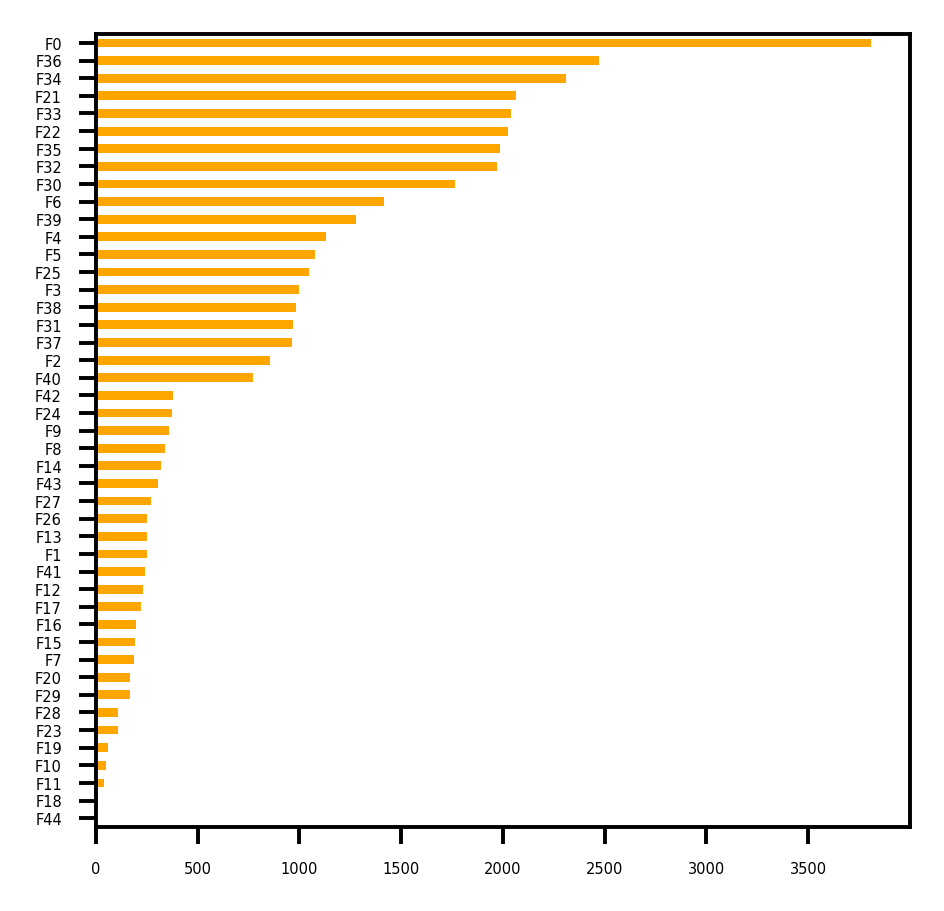
\includegraphics[width=0.45\textwidth,height=90mm]{assets/selectkbest.png}
  \\ Fonte: Condução dos experimentos pelos autores do artigo.
\end{figure}

\subsection{Seleção de Atributos com Base nos Modelos Testados}

Realizamos uma seleção de atributos com base nos modelos \textit{RandomForestClassifier}, \textit{XGBClassifier}, \textit{AdaBoostClassifier} e \textit{LGBMClassifier}, extraindo a média dos valores de \texttt{\footnotesize{feature\_importances\_}} dos modelos.

\begin{figure}[h]
\centering
\caption{\label{figure:figura2}Seleção de Atributos com Base nos Modelos Testados}
  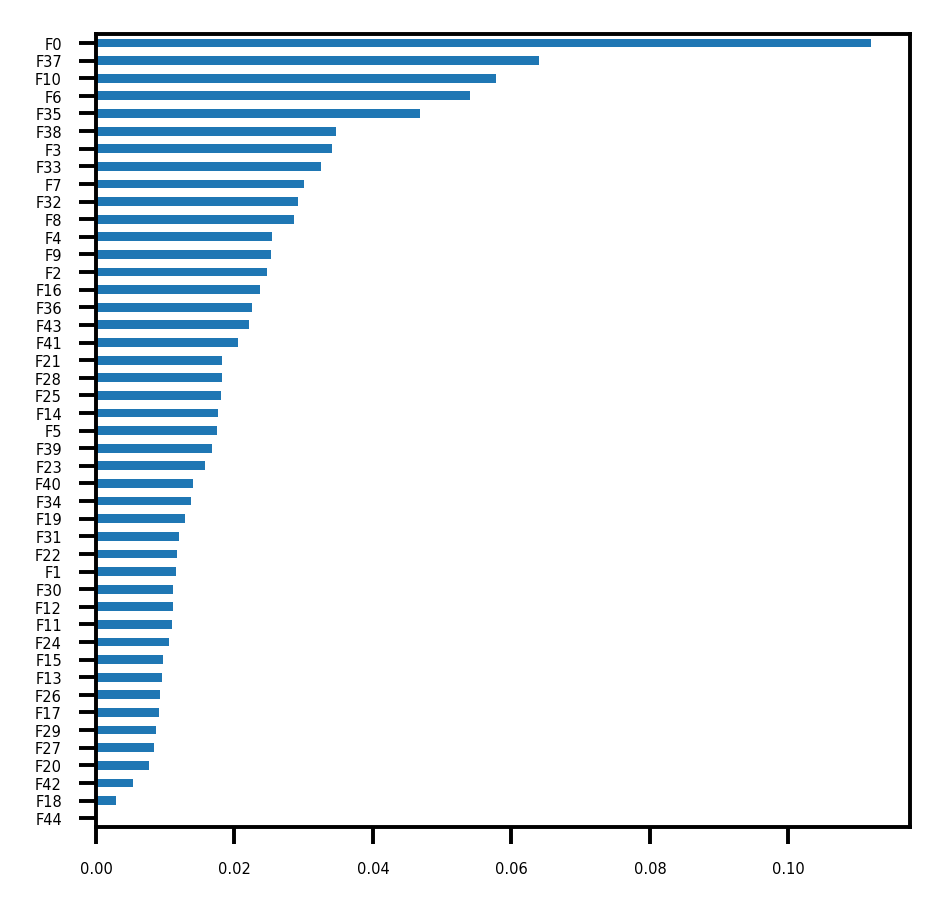
\includegraphics[width=0.45\textwidth,height=90mm]{assets/feature_importances.png}
  \\ Fonte: Condução dos experimentos pelos autores do artigo.
\end{figure}

% \def\code#1{\texttt{#1}}
% \code{\small{RandomForestClassifier}}

\subsection{Resultados dos modelos em Validação}

Tabela 3: Resultados dos Modelos em Validação
\begin{center}
\begin{tabular}{lr}

    \Xhline{2.5\arrayrulewidth}
    \textbf{Classificador} &         \textbf{KS} \\
    \Xhline{2.5\arrayrulewidth}

    \textit{RandomForestClassifier} &  20.730660 \\
    \hline
    \textit{XGBClassifier} &  \textbf{26.341257} \\
    \hline
    \textit{AdaBoostClassifier} &  25.197695 \\
    \hline
    \textit{LogisticRegression} &  18.471405 \\
    \hline
    \textit{LGBMClassifier} &  \textbf{27.209834} \\

\end{tabular}
\\ Fonte: Condução dos experimentos pelos autores do artigo.
\end{center}

Acerca do teste dos modelos \textit{XGBClassifier} e \textit{LGBMClassifier}, obtemos como resultado (KS), respectivamente, 27.1 e 26.9.

\section{Discussão dos Resultados}

Observamos que os modelos \textit{XGBoost} e \textit{LighGBM} tiveram os melhores desempenhos em validação e teste. O \textit{LighGBM} apresenta a vantagem de ser muito mais rápido em treinamento se comparado aos demais modelos, fato esse que é somado com seu maior valor de KS para validação. Contudo, em teste, o \textit{XGBoost} apresentou o melhor resultado (KS de 27.1), sendo a escolha final do modelo.

\begin{figure}[h]
\centering
\caption{\label{figure:figura3}Curvas ROC dos modelos \textit{XGBoost} e \textit{LighGBM}}
  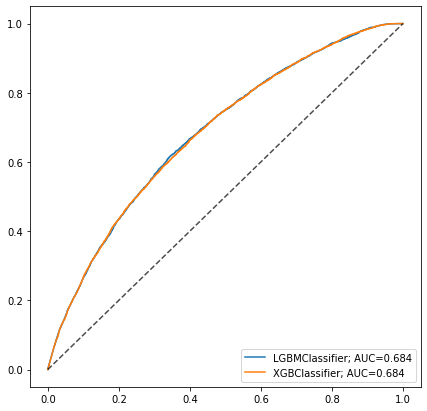
\includegraphics[width=0.4\textwidth,height=70mm]{assets/auc_roc.png}
  \\ Fonte: Condução dos experimentos pelos autores do artigo.
\end{figure}

Plotamos as curvas ROC e o valor de AUC para ambos modelos mencionados, de maneira a entender suas diferenças, apesar da diferença nos valores de KS em teste; as curvas são bem próximas, e possuem o mesmo valor de AUC. De maneira a entender se existem diferenças significativas entre os modelos supracitados, utilizamos o teste \textit{Wilcoxon} (pareado e não paramétrico), conduzindo 10 vezes os experimentos (\textit{k-fold}) com os algoritmos. Ao fim, o teste resultou em um p-valor dacima do limiar estabelecido (5\%), indicando que não existem diferenças significativas entre os modelos treinados. 

\section{Conclusão}

Neste trabalho, buscamos comparar alguns classificadores na tarefa de análise de crédito, de maneira a criar um modelo que apresentasse os melhores resultados da métrica KS para o problema estabelecido. Observamos que os \textit{ensembles} baseados em árvore e com \textit{Gradient Boosting} atingiram os melhores resultados, respectivamente \textit{XGBoost} e \textit{LightGBM}. Também observamos que o \textit{XGBoost} obteve um melhor KS em teste (27.1), apesar de ambos modelos não apresentarem diferença estatística significativa.

Para esse trabalho, foi de fundamental importância o processo de seleção de atributos, de maneira que apenas os filtros não foram suficientes para atingirmos os resultados apresentados. A combinação de atributos importantes para os modelos, bem como atributos importantes para os métodos de filtro, resultaram em melhores valores de KS, uma vez que a combinação de \textit{features} tem o potencial de alavancar melhores resultados, principalmente se realizadas combinações onde os atributos geram bastante informação para a aprendizagem dos modelos.

Em trabalhos futuros, é interessante explorar o processo de \textit{feature engineering}, criando atributos que aumentem os valores de KS para os modelos. Também poderíamos criar uma rede neural para esse problema, passando novas \textit{features} e normalizando os dados; por fim, poderíamos combinar um dos modelos baseados em árvore (\textit{XGBoost} ou \textit{LightGBM}) com a rede criada através de um meta classificador (uma ideia é o \textit{StackingClassifier} do módulo \textit{sklearn}), gerando resultados mais robustos.

\begin{thebibliography}{00}
    \bibitem{b1} Barddal, J., Loezer, L., Enembreck, F., \& Lanzuolo, R. (2020, 30 de dezembro). Lessons learned from data stream classification applied to credit scoring. Elsevier, 162.
    \bibitem{b2} Schölkopf, B., Luo, Z., \& Vovk, V. (Eds.). (2013). Empirical Inference. Springer Berlin Heidelberg.
    \bibitem{b3} M. Chen, Q. Liu, S. Chen, Y. Liu, C. Zhang and R. Liu, "XGBoost-Based Algorithm Interpretation and Application on Post-Fault Transient Stability Status Prediction of Power System," in IEEE Access, vol. 7, pp. 13149-13158, 2019, doi: 10.1109/ACCESS.2019.2893448.
    \bibitem{b4} Lightgbm.readthedocs.io. 2021. LightGBM 3.3.1.99 documentation. [online] Available at: https://lightgbm.readthedocs.io/en/latest/ [Accessed 2 November 2021].
    \bibitem{b5} F. Pedregosa et al., “Scikit-learn: Machine Learning in Python,” Journal of Machine Learning Research, vol. 12, pp. 2825–2830, 2011.
\end{thebibliography}
%\vspace{12pt}

\end{document}